\chapter{Introduction to Nepali Language Model}
\section{Abstract}
This proposal is prepared for development of Nepali Text Generation model and automatic speech recognition of Nepali language. The objective is to enhance the communication and accessibility for Nepali speakers. The project will involve the implementation of machine learning models and the utilization of a large corpus of Nepali text and speech data to train and fine-tune the model. The successful completion of this project will result in the creation of robust and accurate Nepali text generation model which can work as a basis for the development of various other NLP models like Automatic Speech Recognition, Nepali Text Summarization, Question Answering, Content Generation, Paraphrasing, etc. In addition, the development of Automatic Speech Recognition (ASR) for the Nepali language can greatly assist individuals who lack writing skills in effectively conveying their ideas.


\textbf{Keywords: } Nepali Text Generation, Nepali Speech-to-Text, Transformer, LSTM, MFCC


\section{Introduction}
This proposal outlines a project focused on Nepali text generation and Nepali automatic speech recognition. The objective of this endeavor is to develop advanced language processing technologies specifically tailored to the Nepali language, facilitating improved communication, information access, and interaction for Nepali-speaking individuals.

Nepali, as one of the prominent languages in Nepal and various regions of South Asia, holds significant cultural and linguistic importance. However, the availability of robust language processing tools and resources for Nepali remains limited compared to widely studied languages. This project aims to bridge this gap by developing innovative solutions that address the specific linguistic characteristics and challenges of the Nepali language.

The project will primarily focus on two key areas: Nepali text generation and Nepali automatic speech recognition.

\subsection{Nepali Text Generation}
Nepali text generation involves the creation of algorithms and models capable of generating coherent and contextually appropriate Nepali text. This technology holds immense potential in applications such as natural language interfaces, chatbots, content generation, and machine translation systems. By developing advanced techniques for Nepali text generation, we can significantly enhance the quality and efficiency of communication and content creation in Nepali.

\subsection{Nepali Automatic Speech Recognition}
Nepali automatic speech recognition aims to design and develop algorithms and systems that can accurately transcribe spoken Nepali into written text. This technology has the potential to revolutionize various domains, including transcription services, voice-controlled applications, voice assistants, and accessibility tools for individuals with hearing impairments. By leveraging state-of-the-art techniques in speech recognition, we can unlock new opportunities for Nepali speakers to interact with technology and access information more seamlessly.

The successful implementation of this project will require extensive research, data collection, algorithm development, and rigorous evaluation. We will adopt a multidisciplinary approach, combining expertise in natural language processing, machine learning, linguistics, and Nepali language resources.

Furthermore, this project aims to foster collaborations with language experts, academic institutions, industry partners, and native speakers to ensure the authenticity and effectiveness of the developed technologies. Additionally, we will explore avenues for open-source contributions and knowledge sharing, aiming to create a lasting impact in the Nepali language processing community.

By undertaking this project, we aspire to make significant strides in advancing the capabilities of Nepali language processing technologies, empowering Nepali speakers.

\section{Problem Statement}
\begin{enumerate}
    
    \item There is no proper development of various NLP tasks like text generation, text summarization, image captioning, text to speech, etc.\ due to lack of reliable Nepali language model
    \item Nepali Language is rich in vocabulary, and it is difficult to choose the best possible vocab.
    \item Substantial portion of Nepalese population is unable to write properly, despite having clear speech. This issue can be addressed using Nepali ASR.
    \item Transcribing and Documenting the spoken Nepali content is time-consuming and requires greater effort which can be made easier with ASR.
\end{enumerate}

\section{Objectives}
\begin{enumerate}
    \item To develop Nepali language model for text generation.
    \item To develop Nepali Automatic Speech Recognition System.
\end{enumerate}

\section{Project Management}
\begin{figure}[H]
    \centering
    
    \subfigure[Discord]{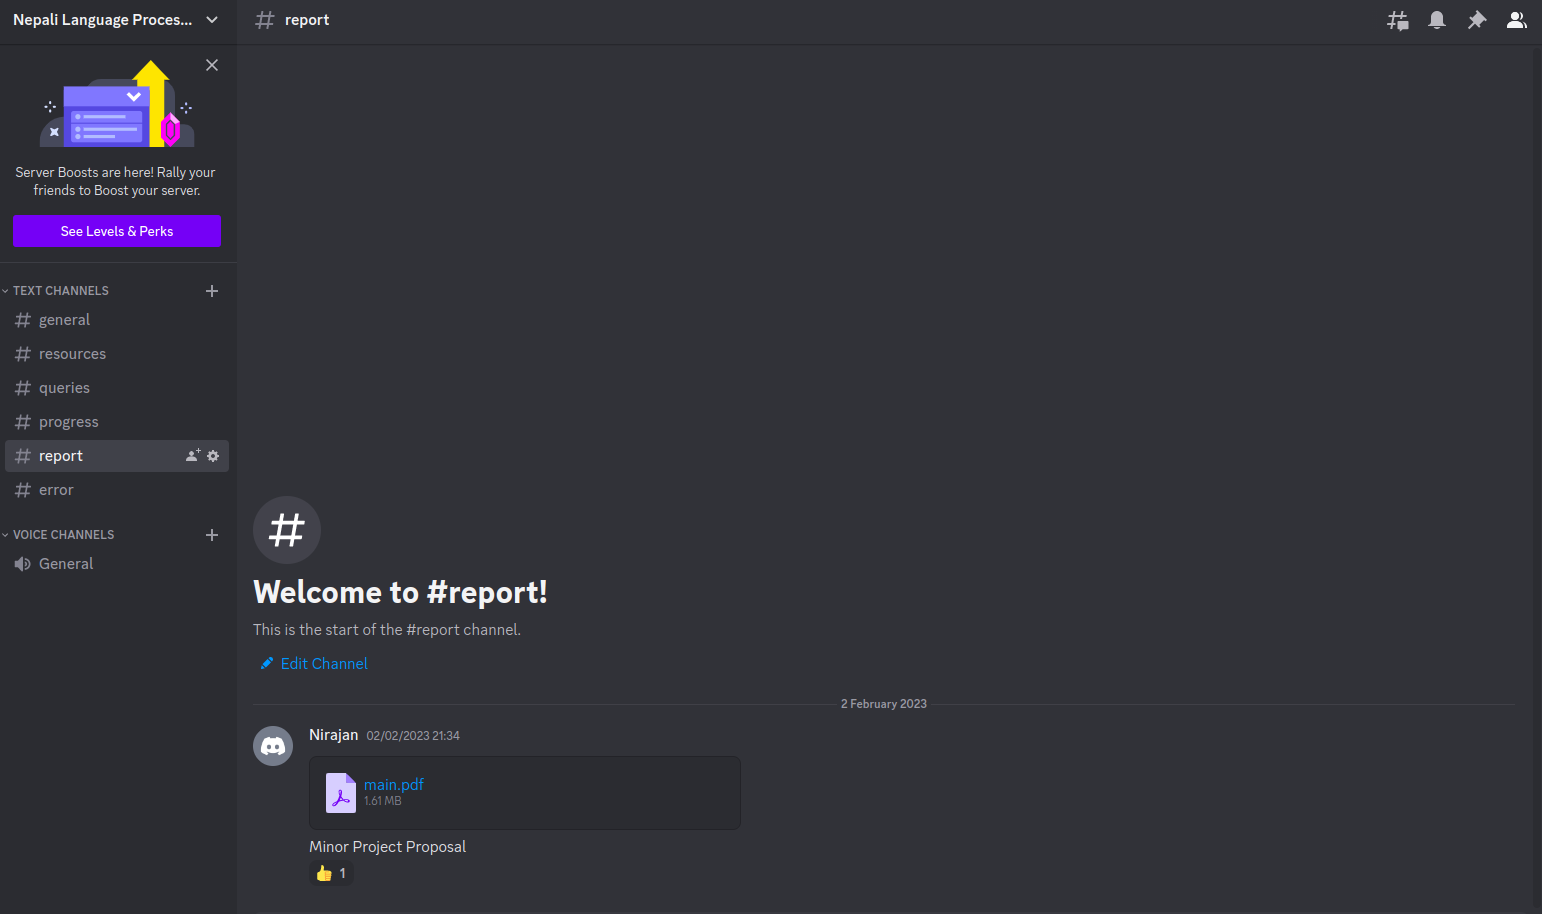
\includegraphics[width=0.45\textwidth]{project_management/discord.png}}
    \subfigure[Trello]{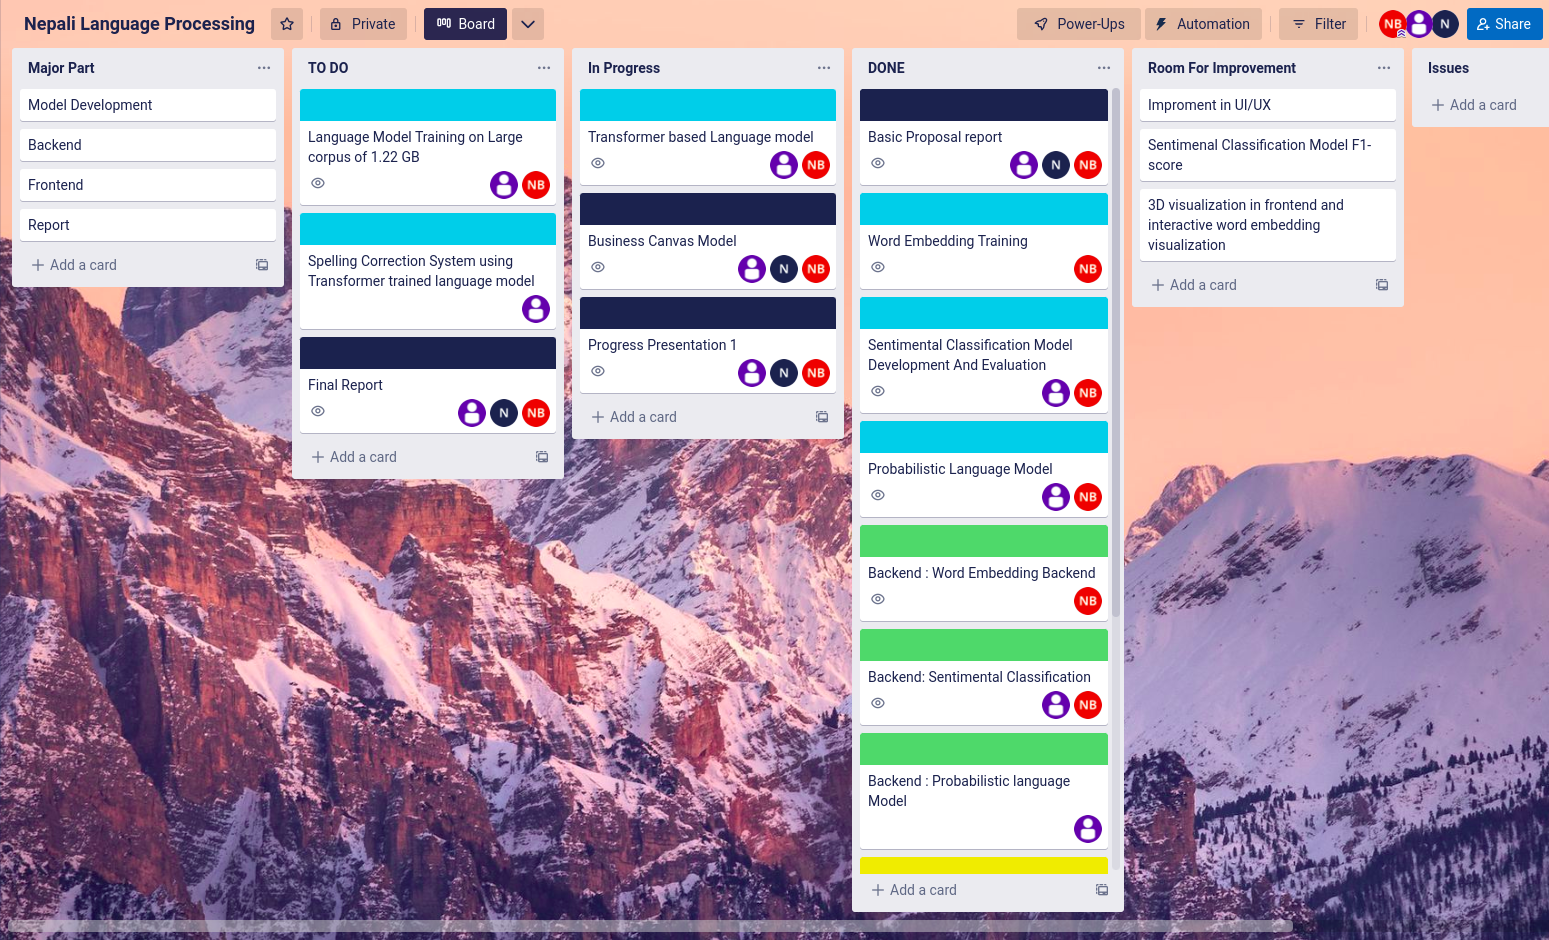
\includegraphics[width=0.45\textwidth]{project_management/trello.png}}//
    \subfigure[Agile Methodology]{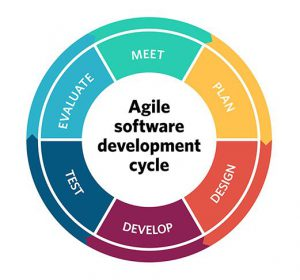
\includegraphics[width=0.45\textwidth]{project_management/agile.jpg}}
    \caption{Project Management}
    \label{fig:my_label}
\end{figure}

Discord will be used as it offers a versatile and user-friendly environment for team communication. Trello will be use as project management tool as it offers a visual and intuitive interface for organizing tasks and tracking project progress. The default agile board will be used for managing this project.


\section{Expected Outcome}
For language generation model, after user input some text, language generation model should suggest next words as shown below.

\begin{figure}[H]
    \centering
    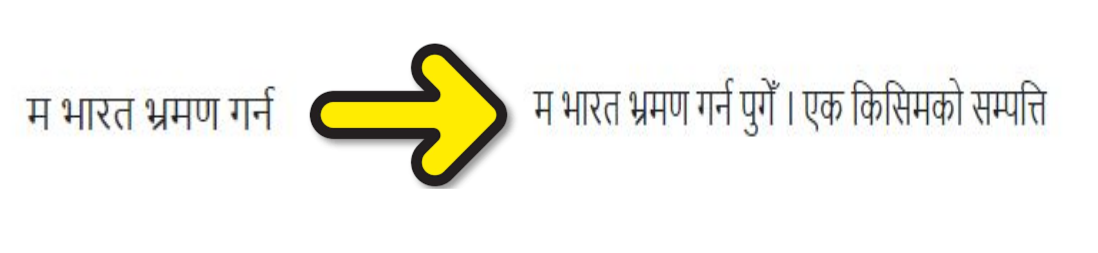
\includegraphics[scale = 0.35]{text_generation.png}
    \caption{Nepali Text Generation}
    \label{fig:Nepali Text Generation}
\end{figure}

And for the Nepali ASR, the model should be able to take Nepali audio as an input and convert it to Nepali text.

